\documentclass[a4paper, 12pt]{mwart}
\usepackage[12pt]{moresize}
\usepackage[T1]{fontenc}
\usepackage{lipsum}
\usepackage{graphicx}
\usepackage[polish]{babel}
\usepackage{array}
\usepackage{cmbright}
\usepackage{polski}
\usepackage{amsmath}

\usepackage[margin = 1.cm]{geometry}

\setlength{\parskip}{4pt}

\setlength{\intextsep}{4pt}

\begin{document}
\pagenumbering{gobble}
	\begin{titlepage}
		\begin{center}
			
\includegraphics[height = 0.6\textheight]{pictures/agh_znk_wbr_rgb_150ppi.jpg}

			\begin{HUGE}
				Metody Obliczeniowe
				i Planowanie Eksperymentu
				\vspace{0.8cm}

				\emph{Projekt 1}
			\end{HUGE}

		\end{center}
		\begin{figure}[b]
			\begin{tabular}{m{4cm}l}
				Imię i nazwisko  & \textbf{Wojciech Brandt}\\
				Number albumu    & \textbf{401 841}\\
				Wydział          & \textbf{Inżynierii Mechanicznej i Robotyki}\\
				Kierunek         & \textbf{Mechanika i Budowa Maszyn}\\
				Grupa Projektowa & \textbf{CP01}
			\end{tabular}
		\end{figure}
	\end{titlepage}

	\section{Cele projektu I}
		Student:
		\begin{itemize}
			\item oswoi się ze sposobem badania układów przed następnym projektem
			\item zapozna się z metodami opracowywania zależności empirycznych i badania ich zgodności
		\end{itemize}

	\section{Badanie wstępne}
		\subsection{Ogólne zachowanie układu}
			W celu zbadania zachowania układu przeprowadzono szereg badań, z różnymi zakresami badanymi.

			Na początek przeprowadznono badania mające na celu uzyskanie wielu punktów w różnych 
			przedziałach czasowych. Ostatecznie w celu zaprezentowania ogólnego działania układu 
			wygenerowano zestaw danych w zakresie czasu $\left< 1;730 \right> s$:
			\begin{figure}[h]
				\begin{center}
					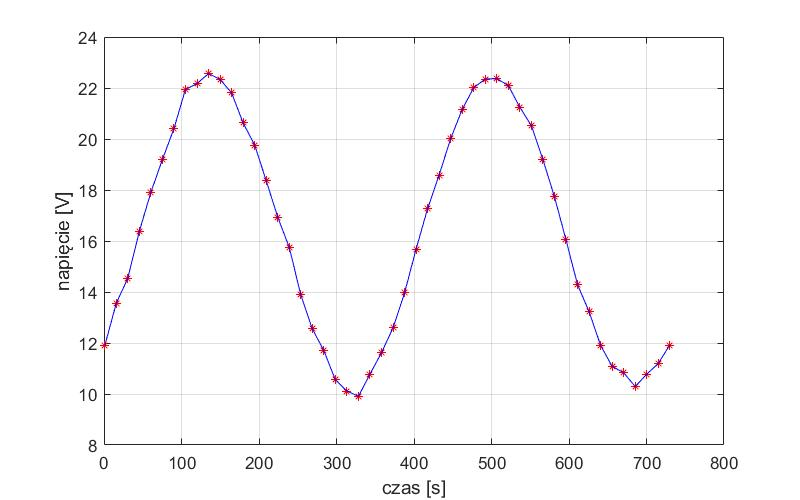
\includegraphics[width = 0.7\linewidth]{graphs/1A.jpg}
					\caption{Dane uzyskane w celu wstępnego określenia działania układu.}
					\label{fig:1A}
				\end{center}
			\end{figure}

			Jak wydać na rys.~\ref{fig:1A} układ zachowuje się w taki sposób, że jego wykres w czasie wygląda 
			podobnie do wykresu funkcji sinusoidalnej. Na wykresie zaznaczone są punkty pomiarowe otrzymane 
			przy pomiarze (zaznaczone czerwonymi gwiazdkami), połączone niebieską linią.

	\newpage
		\subsection{Otrzymywanie danych}
			Dla dalszego określania i obserwowania układu wygenerowano kolejne zestawy danych. Pierwszy z nich
			posłuży w późniejszych etapach do utworzenia modelu matematycznego układu:
			\begin{figure}[h]
				\begin{center}
					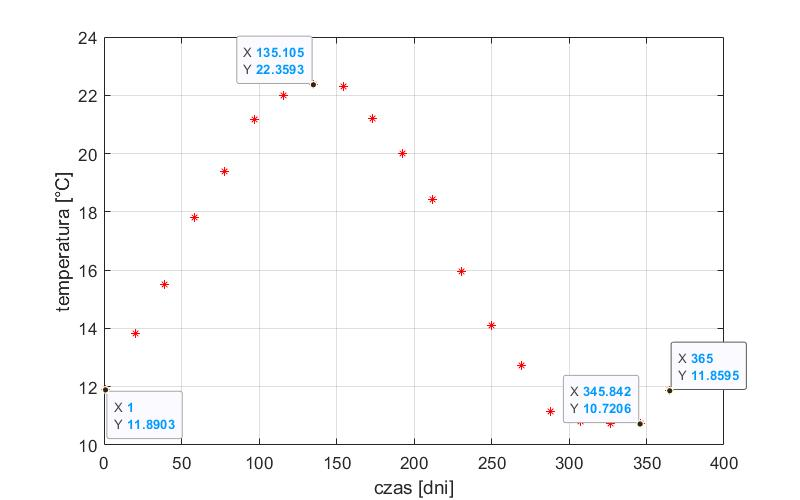
\includegraphics[width = 0.7\linewidth]{graphs/1B-a.jpg}
					\caption{Wykres zestawu danych na którym oparte zostało utworzenie modelu układu.}
					\label{fig:1B}
				\end{center}
			\end{figure}

			A drugi stanowi zestaw danych na podstawie którego możemy określić parametry statystyczne układu:
			\begin{figure}[h]
				\begin{center}
					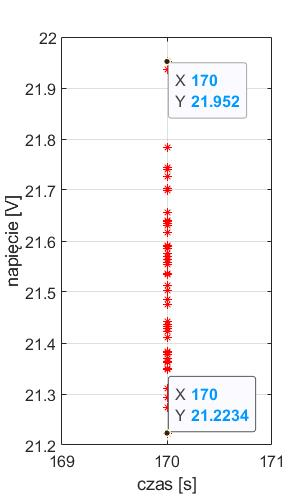
\includegraphics[height = 0.35\textheight]{graphs/1C-a.jpg}
					\caption{Dane otrzymane przy sprawdzaniu wielokrotnie tego samego punktu.}
					\label{fig:1C}
				\end{center}
			\end{figure}

	\newpage
			Z rys.~\ref{fig:1B} odczytać możemy istotne dane dla eksperymentu właściwego:
			\begin{itemize}
				\item Zakres badany: $\left< 1;360 \right>$
				\item Ilość węzłów: $20$
				\item Lokalne maksimum: $V_{max} = 22.596 \text{ V}$
				\item Lokalne minimum: $V_{min} = 10.153 \text{ V}$
			\end{itemize}

			Z rys.~\ref{fig:1C} odczytać możemy istotne dane dla badań wstępnych:
			\begin{itemize}
				\item Czas pomiaru: $170 \text{ s}$
				\item Wartość minimalna: $21.223 \text{ V}$
				\item Wartość maksymalna: $21.952 \text{ V}$
			\end{itemize}

		\subsection{Parametry statystyczne układu}
			
			Na podstawie danych przedstawionych na rys.~\ref{fig:1C} możemy wyznaczyć pewne parametry statystyczne
			układu.

			\begin{description}
				\item[Ilość powtórzeń] wynosi 50.
				\item[Średnia] wyznaczona na podstawie wzoru:
					$$ \bar{x} = \frac{1}{n} \sum_{i=1}^n x_i =  21.5321 \text{ V}$$
				\item[Mediana] wynosi $21.5341 \text{ V}$
				\item[Wariancja] wyznaczona na podstawie wzoru:
					$$ s^2 = \frac{1}{n - 1} \sum_{i=1}^n (y_i - \bar{y})^2 = 0.02648$$
				\item[Odchylenie standardowe] wyznaczone na podstawie wzoru:
					$$ s = \sqrt{\frac{1}{n - 1} \sum_{i=1}^n (y_i - \bar{y})^2} = 0.16272$$
				\item[Histogram]:
					\begin{figure}[h]
						\begin{center}
							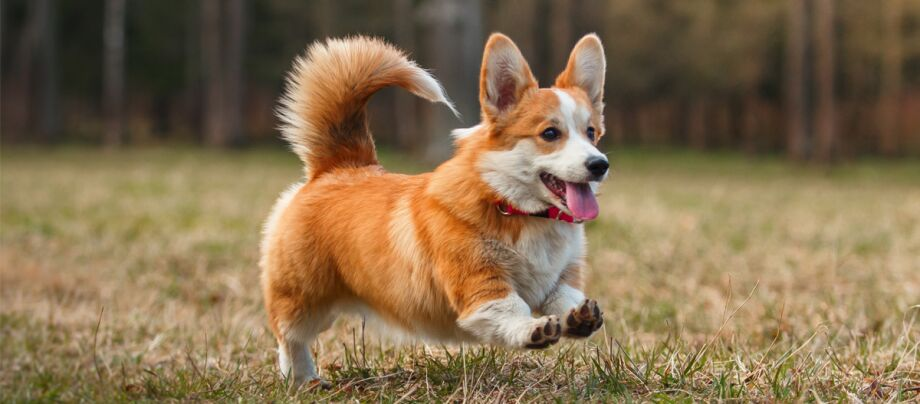
\includegraphics[width = 0.6\textwidth]{pictures/ratgeber_hund_rasse_portraits_welsh-corgi-pembroke_1200x527.jpg}
						\end{center}
					\end{figure}
			\end{description}

	\newpage
	\section{Eksperyment właściwy}
		Dane wejściowe do eksperymentu właściwego przedstawione są na wykresie:
		\begin{figure}[h]
			\begin{center}
				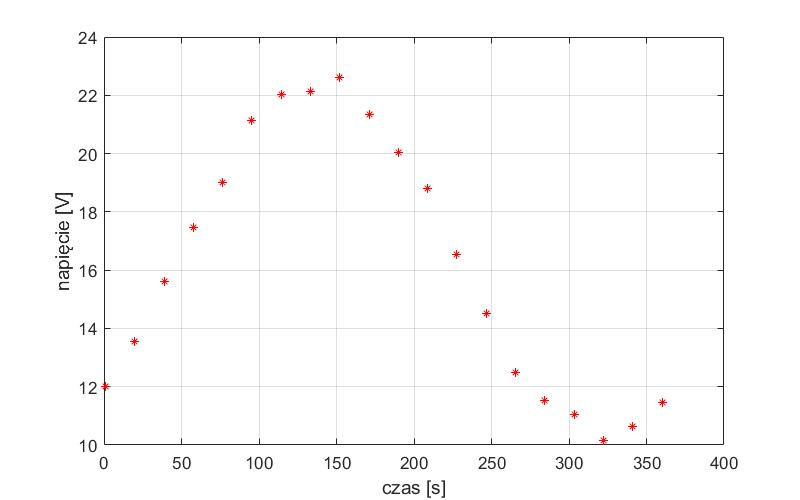
\includegraphics[width = 0.7\textwidth]{graphs/2A.jpg}
				\caption{Wykres danych zmiennych wejściowych dla eksperymentu właściwego}
				\label{fig:2A}
			\end{center}
		\end{figure}

		\subsection{Standaryzacja zmiennych wejściowych}
			Pierwszym krokiem eksperymentu właściwego jest przeskalowanie (standaryzacja)
			danych do\\ przedziału $\left\langle -1; 1 \right\rangle$. Wykonano to za pomocą obliczenia:
			\begin{description}
				\item[średniej] ze wzoru:
					$$\bar{x} = \frac{x_{i,min} + x_{i,max}}{2}$$
				\item[jednostki zmienności] ze wzoru:
					$$\Delta x = \frac{x_{i,max} + x_{i,min}}{2}$$
				\item[Oraz podstawienia] powyższych wraz z kolejnymi wartościami $x_i$ do wzoru:
					$$t_i = \frac{x_i - \bar{x}}{\Delta x}$$
			\end{description}
			
			\newpage
			A więc dane z rys.~\ref{fig:2A} przedstawione wobec nowej osi zmiennej standaryzowanej
			prezentują\\się następująco:
			\begin{figure}[h]
				\begin{center}
					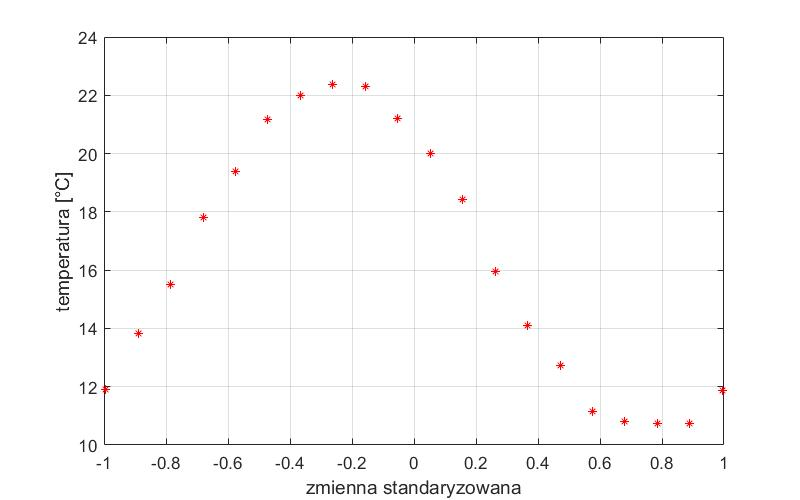
\includegraphics[width = 0.7\textwidth]{graphs/2B.jpg}
					\caption{Zmienne wejściowe przedstawione wobec osi $x$ standaryzowanej}
					\label{fig:2B}
				\end{center}
			\end{figure}

		\subsection{Opracowanie modelu badań}
			Model układu utworzony zostanie poprzez wykorzystanie aproksymacji średniokwadratowej.
			Uogólniony wzór funkcji aproksymującej wyglada w następujący sposób:
			$$ Q(x) = a_1 q_1(x) + a_2 q_2(x) + ... + a_j q_j(x) + ... a_m q_m(x) = \sum_{j=1}^m a_j q_x(x)$$
			gdzie $q_j(x)$ jest obraną funkcją bazową, a współczynniki $a_i$ wyznaczać będziemy ze
			wzoru macierzowego:
			$$ \textbf{A} = \left( \textbf{X}^T \cdot \textbf{X} \right)^{-1} \cdot \textbf{X}^T \cdot \textbf{Y} $$

			\subsubsection{Aproksymacja funkcją wielomianową}
				Wzór ogólny dla aproksymacji funkcjami wielomianowymi wygląda następująco:
				$$ Q(x) = a_1 + a_2x + a_3 x^2 + a_4 x^3 + \dots + a_n x^{n-1} $$
				
				I w celu określenia dobrego modelu dla układu można sprawdzać różne stopnie $n$, 
				na przykład $n=0$, co da nam funkcję stałej, $n=1$ co da nam prostą, $n=7$ co dam nam
				nam wielomian siódmego stopnia.

				Macierze aproksymacji wyglądać będą więc w następujący sposób:

				$$ \textbf{X} = \begin{bmatrix}
					1      & x_1    & \cdots & x_1^{n-1} \\
					1      & x_2    & \cdots & x_2^{n-1} \\
					\vdots & \vdots &        & \vdots\\ 
					1      & x_n    & \cdots & x_n^{n-1}
				\end{bmatrix} 
				\quad 
				\textbf{A} = \begin{bmatrix}
					a_1\\
					a_2\\
					\vdots\\
					a_n
				\end{bmatrix} \quad
				\textbf{Y} = \begin{bmatrix}
					y_1\\
					y_2\\
					\vdots\\
					y_n
				\end{bmatrix}$$

				\newpage
				\paragraph{Aproksymacja wielomianem 1-go stopnia}

					Otrzymana ze skryptu macierz $\textbf{A}$, wyliczona w oparciu o oś X wejściową:
					$$ \textbf{A} = \begin{bmatrix}
						19.641\\
						-0.019
					\end{bmatrix} $$

					Funkcja aproksymująca:
					$$ Q(x) = 19.641 - 0.019x $$

					Otrzymana ze skryptu macierz $\textbf{B}$, wyliczona w oparciu o
					oś T standaryzowaną:
					$$ \textbf{B} = \begin{bmatrix}
						16.204\\
						-3.437
					\end{bmatrix} $$

					Funkcja aproksymująca:
					$$ Q(x) = 16.204 - 3.437x$$

				\paragraph{Aproksymacja wielomianem 2-go stopnia}

					Otrzymana ze skryptu macierz $\textbf{A}$:
					$$\textbf{A} = \begin{bmatrix}
						13.503\\
						0.088\\
						-0.001
					\end{bmatrix}$$
					
					Funkcja aproksymująca: 
					$$ Q(x) = 13.503 + 0.088x - 0.001x^2 $$

					Otrzymana ze skryptu macierz $\textbf{B}$:
					$$\textbf{B} = \begin{bmatrix}
						19.723\\
						-3.437\\
						-9.656
					\end{bmatrix}$$

					Funkcja aproksymująca:
					$$ Q(x) = 19.723 - 3.437x - 9.656x^2$$

				\paragraph{Aproksymacja wielomianem 7-go stopnia}

					Otrzymana ze skryptu macierz $\textbf{A}$:
					$$\textbf{A} = \begin{bmatrix}
						11.907\\
						0.084\\
						1\cdot 10^{-4}\\
						6\cdot 10^{-6}\\
						-1.015\cdot 10^{-7}\\
						5 \cdot 10^{-10}\\
						0\\
						5.286
					\end{bmatrix}$$

					Funkcja aproksymująca (w przybliżeniu):
					$$ Q(x) \approx 11.907 + 0.084x + 5.286 x^7 $$

					Otrzymana ze skryptu macierz $\textbf{B}$:
					$$\textbf{B} = \begin{bmatrix}
						20.911\\
						-12.849\\
						-22.03\\
						22.272\\
						17.803\\
						-12.926\\
						-4.981\\
						3.3
					\end{bmatrix}$$

					Funkcja aproksymująca:
					$$ Q(x) = 20.911 - 12.849x - 22.03x^2 + 22.272x^3 + 17.803x^4 - 12.926x^5 - 4.981x^6 + 3.3x^7 $$


				\paragraph{Otrzymane funkcje} prezentują się w następujący sposób:

					Dla zmiennej wejściowej (na podstawie funkcji o współczynnikach macierzy $\textbf{A}$):
					\begin{figure}[h]
						\begin{center}
							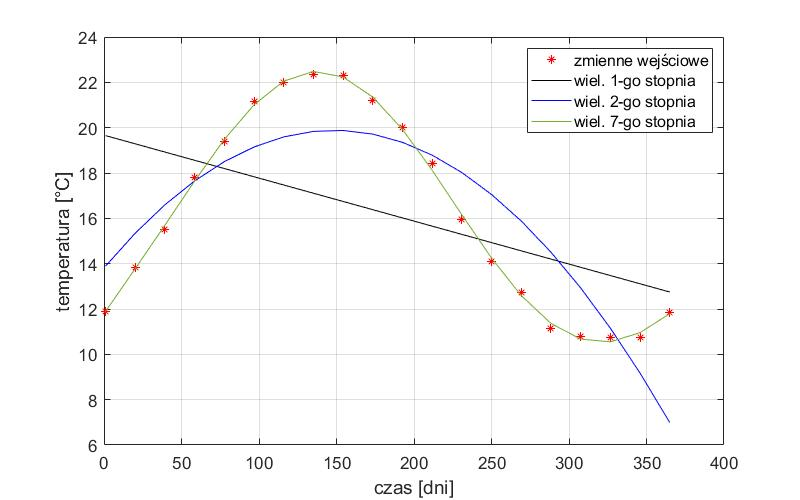
\includegraphics[width = 0.7\textwidth]{graphs/3-n.jpg}
							\caption{Wyniki aproksymacji wielomianami wobec osi zmiennych wejściowych}
							\label{fig:3N}
						\end{center}
					\end{figure}

					Dla zmiennej standaryzowanej (na podstawie funkcji o współczynnikach macierzy $\textbf{B}$):
					\begin{figure}[h]
						\begin{center}
							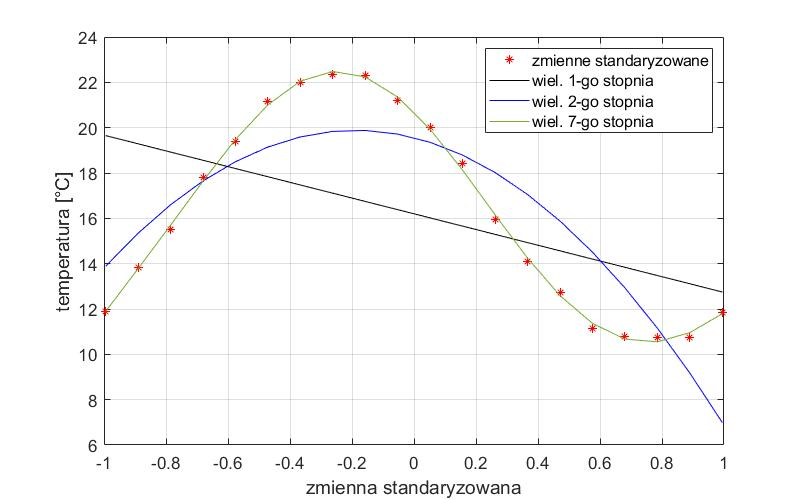
\includegraphics[width = 0.7\textwidth]{graphs/3-s.jpg}
							\caption{Wyniki aproksymacji wielomianami wobec osi zmiennych standaryzowanych}
							\label{fig:3S}
						\end{center}
					\end{figure}

			\newpage
			\subsubsection{Aproksymacja funkcją logarytmu naturalnego}
				Wzór uogólniony aproksymacji jest następujący:

				$$ Q(x) = a_1 + a_2 \ln\left(x\right) + a_3\ln^2\left(x\right) + \dots + a_n \ln^{n-1} \left(x\right)$$

				A macierze aproksymacji prezentują się w następujący sposób:
	
				$$ \textbf{X} = \begin{bmatrix}
					1      & \ln \left(x_1\right) & \cdots & \ln^{n-1} \left(x_1\right)\\
					1      & \ln \left(x_2\right) & \cdots & \ln^{n-1} \left(x_2\right)\\
					\vdots & \vdots               &        & \vdots \\
					1      & \ln \left(x_n\right) & \cdots & \ln^{n-1} \left(x_n\right)
				\end{bmatrix}
				\quad 
				\textbf{A} = \begin{bmatrix}
					a_1\\
					a_2\\
					\vdots\\
					a_n
				\end{bmatrix} \quad
				\textbf{Y} = \begin{bmatrix}
					y_1\\
					y_2\\
					\vdots\\
					y_n
				\end{bmatrix}$$	

				Na tym etapie należy zaznaczyć, że niemożliwe jest aproksymowanie funkcją logarytmu
				naturalnego w oparciu o zmienne standaryzowane, gdyż nie istnieje logarytm z wartości
				ujemnej.

				Macierz $\textbf{A}$ otrzymana ze skryptu:

				$$\textbf{A} = \begin{bmatrix}
					12.015\\
					254.938\\
					-238.544\\
					81.3\\
					-11.922\\
					0.636
				\end{bmatrix}$$

				A więc funkcja aproksymująca:
				$$Q(x) = 12.015 + 254.938 \ln \left(x\right) - 238.544 \ln^2 \left(x\right)
				+ 81.3 \ln^3 \left(x\right) - 11.922 \ln^4 \left(x\right) + 0.636 \ln^5 \left(x\right)$$

				I jej wykres:
				\begin{figure}[h]
					\begin{center}
						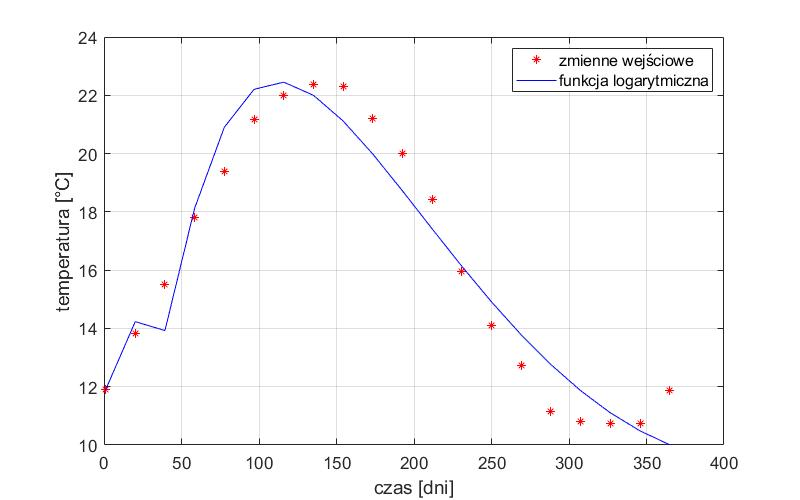
\includegraphics[width = 0.7\textwidth]{graphs/4-n.jpg}
					\end{center}
				\end{figure}

				Jak widać przy programowaniu skryptu zdecydowano się na przyjęcie stopnia $n=6$.
				Wybór ten wynika z nieadekwatności modelu do układu - dalsze zwiększanie współczynnika dawało
				niewiele lepsze rezultaty.

		\newpage
			\subsubsection{Aproksymacja funkcją wymierną}
				Wzór uogólniony funkcji jest następujący:
				$$Q(x) = a_1 + a_2 \left(\frac{1}{x}\right) + a_3 \left(\frac{1}{x}\right)^2 + \dots + a_n \left(\frac{1}{x}\right)^{n-1}$$

				A macierze aproksymujące są następujące:
				$$\textbf{X} = \begin{bmatrix}
					1     & \frac{1}{x_1} & \cdots & \left(\frac{1}{x_1}\right)^{n-1}\\
					1     & \frac{1}{x_2} & \cdots & \left(\frac{1}{x_2}\right)^{n-1}\\
					\vdots& \vdots        &        & \vdots\\
					1     & \frac{1}{x_n} & \cdots & \left(\frac{1}{x_n}\right)^{n-1}\\
				\end{bmatrix}
				\quad 
				\textbf{A} = \begin{bmatrix}
					a_1\\
					a_2\\
					\vdots\\
					a_n
				\end{bmatrix} \quad
				\textbf{Y} = \begin{bmatrix}
					y_1\\
					y_2\\
					\vdots\\
					y_n
				\end{bmatrix}$$

				Macierz $\textbf{A}$ otrzymana ze skryptu:
				$$\textbf{A} = \begin{bmatrix}
					-7.576\\
					8.137 \cdot 10^3\\
					-7.208 \cdot 10^5\\
					2.345 \cdot 10^7\\
					-2.536 \cdot 10^8\\
					2.309 \cdot 10^8
				\end{bmatrix}$$

				Funkcja aproksymująca:
				$$Q(x) = -7.576  + 8.137 \cdot 10^3 \cdot \frac{1}{x} -7.208 \cdot 10^5 \cdot
				\left(\frac{1}{x}\right)^2 + 2.345 \cdot 10^7 \cdot \left(\frac{1}{x}\right)^3
				-2.536 \cdot 10^8 \cdot \left(\frac{1}{x}\right)^4 + 2.309 \cdot 10^8 \cdot \left(
				\frac{1}{x}\right)^5$$

				Macierz $\textbf{B}$ otrzymana ze skryptu:
				$$\textbf{B} = \begin{bmatrix}
					13.906\\
					-1.694\\
					0.227\\
					0.039\\
					-5.724 \cdot 10^{-4}\\
					-9.551 \cdot 10^{-5}
				\end{bmatrix}$$
				
				Funkcja aproksymująca:
				$$Q(x) = 13.906 - 1.694\cdot \frac{1}{x} + 0.227\cdot
				\left(\frac{1}{x}\right)^2 + 0.039\cdot \left(\frac{1}{x}\right)^3 
				 -5.724\cdot 10^{-4}\cdot \left(\frac{1}{x}\right)^4   -9.551 \cdot 10^{-5}\cdot 
				 \left(\frac{1}{x}\right)^5$$

			\newpage
				Wykres funkcji aproksymującej na podstawie współczynników otrzymanych w oparciu
				o oś zmiennych wejściowych $\textbf{x}$:
				\begin{figure}[h]
					\begin{center}
						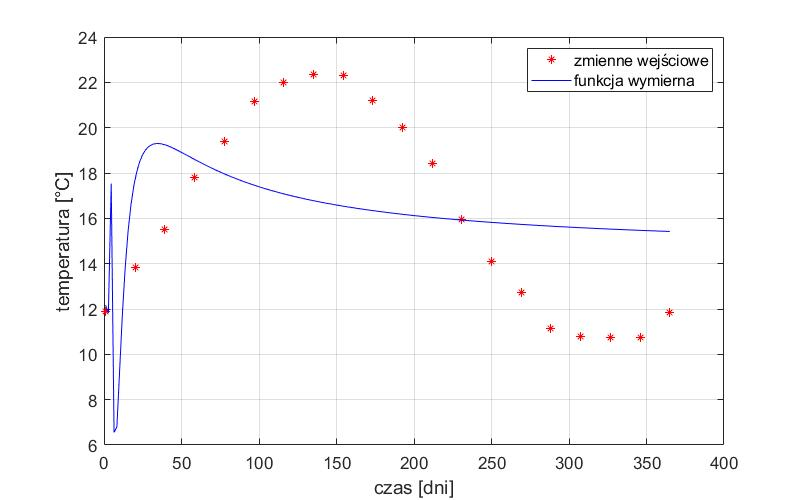
\includegraphics[width = 0.7\textwidth]{graphs/5-n.jpg}
						\caption{Wykres aproksymacji funkcją wymierną na zmiennych wejściowych}
						\label{fig:5n}
					\end{center}
				\end{figure}

				Wykres funkcji aproksymującej na podstawie współczynników otrzymanych w oparciu
				o oś zmiennych standaryzowanych $\textbf{t}$:
				\begin{figure}[h]
					\begin{center}
						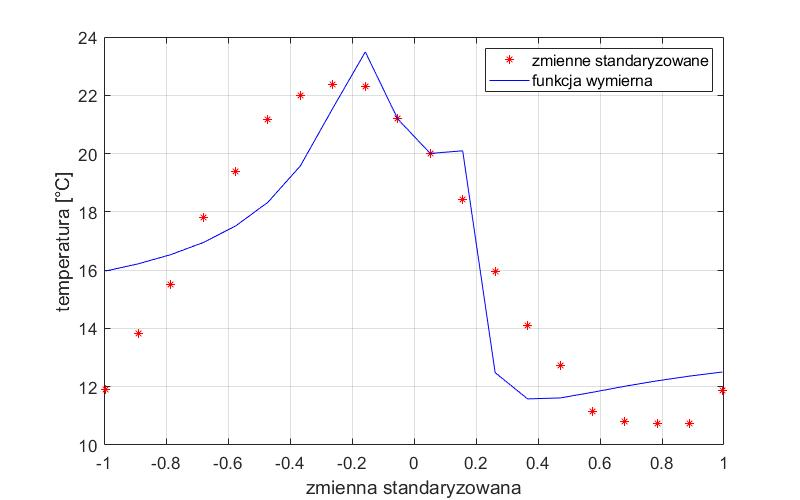
\includegraphics[width = 0.7\textwidth]{graphs/5-s.jpg}
						\caption{Wykres aproksymacji funkcją wymierną na zmiennych standaryzowanych}
						\label{fig:5s}
					\end{center}
				\end{figure}

			\subsubsection{Aproksymacja funkcją trygonometryczną}
				Wzór uogólniony wybranej funkcji ma następującą postać:
				$$Q(x) = a_1 + a_2 \cos(c\cdot x) + a_3 \sin (c\cdot x) + a_4 \cos(c\cdot 2x)
				+ a_5 \sin (c\cdot 2x) +\dots + a_n \cos (c\cdot \frac{n}{2}x) + 
				a_{n+1} \sin(c \cdot \frac{n}{2}x)$$

				Gdzie $c$ to zmienna mająca wpływ na okres funkcji aproksymowanej; podczas prób
				aproksymacji dobierana była empirycznie.

				Macierz aproksymacji $\textbf{X}$ przyjmie postać:
				$$\textbf{X} = \begin{bmatrix}
					1     & \cos(c\cdot x_1) & \sin(c\cdot x_1) & \cdots & \cos(c\cdot \frac{n}{2} x_1) & \cos(c\cdot \frac{n}{2} x_1)\\
					1     & \cos(c\cdot x_2) & \sin(c\cdot x_2) & \cdots & \cos(c\cdot \frac{n}{2} x_2) & \cos(c\cdot \frac{n}{2} x_2)\\
					\vdots& \vdots & \vdots &  & \vdots & \vdots\\
					1     & \cos(c\cdot x_n) & \sin(c\cdot x_n) & \cdots & \cos(c\cdot \frac{n}{2} x_n) & \cos(c\cdot \frac{n}{2} x_n)\\
				\end{bmatrix}$$

				Podczas aproksymacji w oparciu o zmienne wejściowe
				$x$ wybrano współczynnik $c=0.003\cdot \pi$. \\Macierz $\textbf{A}$ otrzymana ze skryptu:
				$$\textbf{A} = \begin{bmatrix}
					15.116\\
					0.746\\
					2.758\\
					-3.881\\
					2.309
				\end{bmatrix}$$

				Postać funkcji aproksymującej:
				$$Q(x) = 15.116 + 0.746 \cos\left(c\cdot x\right) + 2.758 \sin \left(c\cdot x\right)
				- 3.881 \cos \left(c\cdot 2x\right) + 2.309 \sin \left(c \cdot 2x\right)$$

				Podczas aproksymacji w oparciu o zmienne standaryzowane $t$ wybrano współczynnik 
				$c=\pi$. \\Macierz $\textbf{B}$ otrzymana ze skryptu:
				$$\textbf{B} = \begin{bmatrix}
					16.409\\
					4.531\\
					-4.048\\
					-0.0442\\
					0.0145
				\end{bmatrix}$$

				Postać funkcji aproksymującej:
				$$Q(x) = 16.409 + 4.531 \cos\left(c\cdot x\right) - 4.048 \sin \left(c\cdot x\right)
				- 0.0442 \cos \left(c\cdot 2x\right) + 0.0145 \sin \left(c \cdot 2x\right)$$

				Wykres funkcji aproksymującej na podstawie współczynników otrzymanych w oparciu
				o oś zmiennych wejściowych $x$:
				\begin{figure}[h]
					\begin{center}
						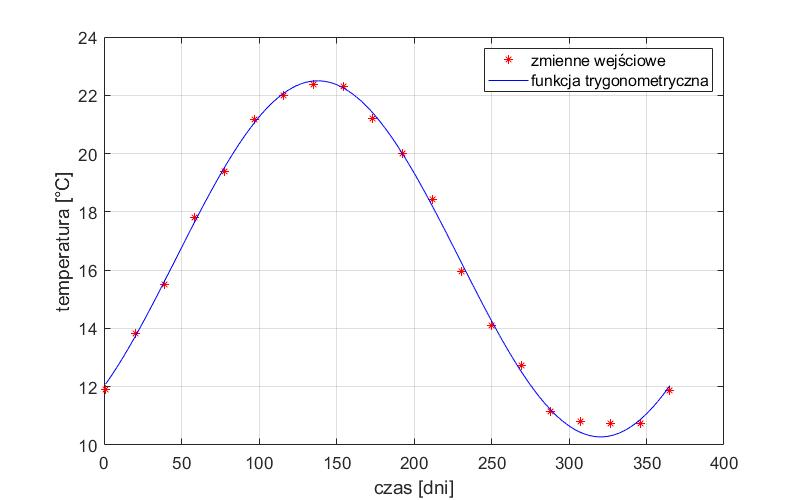
\includegraphics[width = 0.7\textwidth]{graphs/6-n.jpg}
						\caption{Wykres aproksymacji funkcją trygonometryczną na zmiennych wejściowych}
						\label{fig:6n}
					\end{center}
				\end{figure}
			\newpage
				Wykres funkcji aproksymującej na podstawie współczynników otrzymanych w oparciu
				o oś zmiennych standaryzowanych $t$:
				\begin{figure}[h]
					\begin{center}
						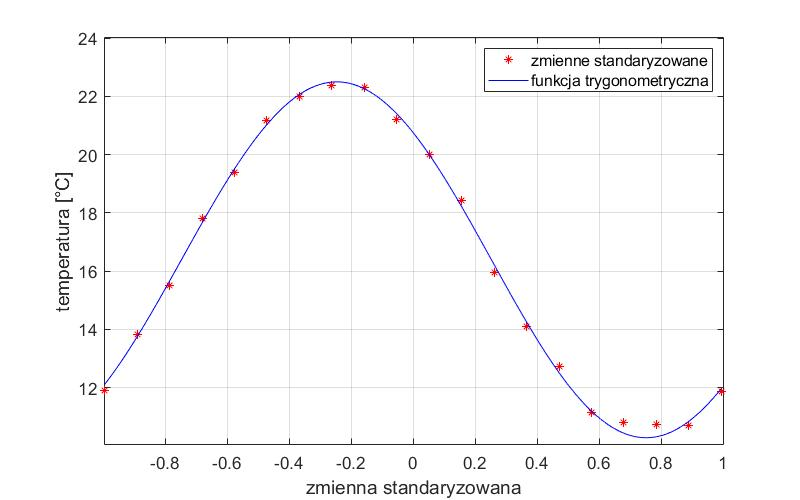
\includegraphics[width = 0.7\textwidth]{graphs/6-s.jpg}
						\caption{Wykres aproksymacji funkcją trygonometryczną na zmiennych standaryzowanych}
						\label{fig:6s}
					\end{center}
				\end{figure}
\end{document}